%!TEX root = ../main.tex

\newpage

\section{Utility Functions for Tgeometry and Rtransform Types}
\label{section:utility_rtransform}

Before diving into the implementation of the general MoblityDB functions that have to be adapted to handle moving regions as well as all the types already present, we will first talk about a set of functions specific to the tgeometry and rtransform types.

These functions can be called utility functions, since they are not presented to the user as an SQL function, but they are used in the backend a lot to simplify other functions. Table \ref{table:rtransform_functions} shows a list of these functions with their signature (input and output types).

\begin{table}[h!]
    \centering
    \begin{tabular}[c]{|l|l|} 
    \hline
    \textbf{Functions}  & \textbf{Signature} \\ 
    \hline
    compute             & polygon    x polygon              $\rightarrow$ rtransform \\
    apply               & rtransform x polygon              $\rightarrow$ polygon \\
    \hline
    interpolate         & rtransform x rtransform x double  $\rightarrow$ rtransform \\
    interpolate long    & rtransform x rtransform x double  $\rightarrow$ rtransform \\
    \hline
    combine             & rtransform x rtransform           $\rightarrow$ rtransform \\
    diff                & rtransform x rtransform           $\rightarrow$ rtransform \\
    \hline
    \end{tabular}
    \caption{Utility functions for the \textit{rtransform} type}
    \label{table:rtransform_functions}
\end{table}

\subsection{Compute}
\label{section:compute}

The \textit{compute} function takes two polygon values as input and computes the transformation from the first to the second one. For example, taking the two polygons shown below as input, with the blue polygon being the first argument and the red polygon being the second, the resulting rtransform will be $\mathcal{T}:\ (1,\ \frac{1}{3},\ \frac{-\pi}{2})$.

\begin{figure}[h!]
    \centering
    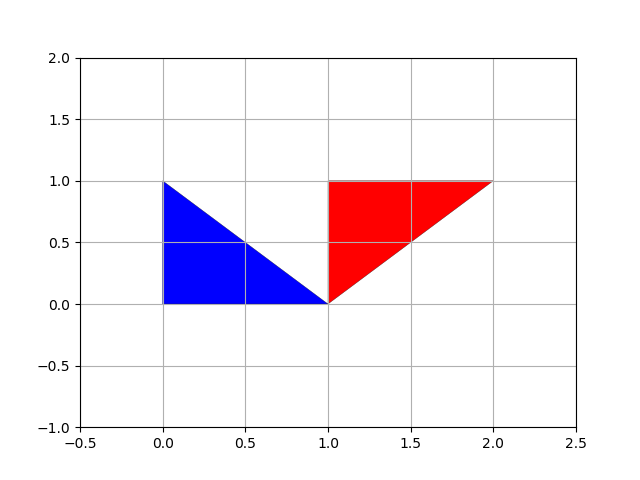
\includegraphics[width=0.6\textwidth]{images/example_simple_transformation.png}
    \caption{Example polygons used in the \textit{compute} function}
    \label{fig:example_compute}
\end{figure}


As said previously the type used to represent a region value is the PostGIS type \textit{Geometry(Polygon)}. This polygon type is defined using rings: one outer ring, and zero or more inner rings defining holes in the polygon. One assumption that we make when receiving the polygons as input is that two polygons of the same shape have their corresponding points defined at the same position in the rings of said polygons. 

The rings are defined as lists of points, with the first and the last points being equal to denote that the ring is closed. Our previous assumption thus says that the $i$'th point in the list defining the outer ring of the first polygon, has to correspond to the $i$'th point in the list defining the outer ring of the second polygon, after application of the correct transformation.

Essentially this means that the points of the polygons are 'numbered' in the same way. This allows us for example to distinguish a square from its 90 degree rotations. \\

The combination of a rotation by $\theta$ around the origin, followed by a translation by $(v^x,\ v^y)$, can be described using a matrix multiplication.

\[
    \begin{bmatrix}
    x' \\
    y' \\ 
    1  \\       
    \end{bmatrix}
    =
    \begin{bmatrix}
    \cos(\theta) & \sin(\theta)  & v^x \\
    \sin(\theta) & -\cos(\theta) & v^y \\ 
    0            & 0             & 1   \\       
    \end{bmatrix}
    *
    \begin{bmatrix}
    x \\
    y \\ 
    1 \\       
    \end{bmatrix}
\]

Using the notation

\[
    \begin{cases}
        a = \cos(\theta) \\
        b = \sin(\theta) \\
        c = v^x          \\
        d = v^y          \\
    \end{cases}
\]

, and by taking the first two points of the outer rings of both input polygons, we have the following list of equations:

\[
    \begin{cases}
        a*x_1 - b*y_1 + c = x_1' \\
        a*y_1 + b*x_1 + d = y_1' \\
        a*x_2 - b*y_2 + c = x_2' \\
        a*y_2 + b*x_2 + d = y_2' \\
    \end{cases}
\]

, with $(x_1, y_1)$ and $(x_2, y_2)$ being the first two points of the first polygon, and $(x_1', y_1')$ and $(x_2', y_2')$ being the corresponding points on the second polygon.

We can then solve these equations for $a$, $b$, $c$ and $d$.

\[
    \begin{cases}
        a = \frac{(x_1' - x_2')*(x_1 - x_2) + (y_1' - y_2')*(y_1 - y_2)}{(x_1 - x_2)^2 + (y_1 - y_2)^2}\\
        b = \frac{(y_1' - y_2')*(x_1 - x_2) - (x_1' - x_2')*(y_1 - y_2)}{(x_1 - x_2)^2 + (y_1 - y_2)^2}\\
        c = x_1' - a*x_1 + b*y_1 \\
        d = y_1' - a*y_1 - b*x_1 \\
    \end{cases}
\]

And finally we can get the parameters of the transformation.

\[
    \begin{cases}
        \theta = atan2(b,\ a) \\
        v^x = c \\
        v^y = d \\
    \end{cases}
\]

As said previously, this computes a transformation which is the combination of first a rotation $\theta$ applied around the origin, and then a translation $(v^x,\ v^y)$. To use these equations, we thus need the centroid of the first polygon (the center of rotation for this transformation) to be at the origin. To solve this issue, we first compute the centroid of the first region, then translate both regions using the same translation, to have the new centroid of the first region be at the origin. Finally we can use the above equations to compute the parameters of the transformations.

When we also need to verify that both input polygons have the same shape, we can apply this computed transformation to the start polygon, and compare all corresponding points with the end polygon after the transformation. If the distance between the position of two corresponding points differs by more than a given $\epsilon$, we can assume that the two regions do not have the same shape.

\subsection{Apply}
\label{section:apply}

This \textit{apply} function does the opposite of the \textit{compute} function. Given an rtransform, and a start polygon, it applies the transformation to retrieve the end polygon. This is done using a PostGIS function called \textit{ST\_Affine}, which applies an affine transformation to the given geometry. 

Applying an affine transformation again means rotating around the origin, so we first have to translate the polygon to have its centroid at the origin, then we can apply the given transformation, and finally we apply the inverse of the first translation to get the final polygon.

\note{Maybe equations or examples?}

\subsection{Interpolate}
\label{section:interpolate}

This function is used when we have a polygon defined at time $t_1$ and another one defined at time $t_2$, and we want to retrieve the position of the polygon at time $t$, where $t_1 < t < t_2$ using linear interpolation. Of course, when using stepwise interpolation this function is not needed, since, if we are looking for the polygon at time $t$, where $t_1 < t < t_2$, the needed polygon is simply the one defined at time $t_1$.

If we wanted to interpolate two polygons using linear interpolation between their vertices, we would not keep the fixed-shape aspect of the polygon, as is in Figure \ref{fig:vertices_interpolation}. For this reason, the interpolation is done on the rtransforms defining the position of the polygon at times $t_1$ and $t_2$ with respect to a certain reference polygon.

For example, using a tgeometryseq with three instants defined at times $t_0$, $t_1$ and $t_2$

\[
    '[\mathcal{R}_0@t_0,\ \mathcal{T}_1@t_1,\ \mathcal{T}_2@t_2]'
\]

, suppose that we want to compute the position of the region at time $t_1 < t < t_2$. To do this, we first apply the \textit{interpolate} function with $\mathcal{T}_1$ and $\mathcal{T}_2$ a arguments, and then apply the resulting rtransform to $\mathcal{R}_0$ to get the result.

The \textit{interpolate} functions takes three input arguments. The first two arguments are the initial and final rtransform values. The third argument is a \textit{ratio} value defined by the timestamp of the resulting rtransform. This ratio is always between 0 and 1, and is computed as follows.

\[
    ratio = \frac{t - t_1}{t_2 - t_1}
\]

Since we assume linear interpolation between the rtransform values, we will simply use linear interpolation to compute the resulting translation value.

\[
    \begin{cases}
        v^x = v_1^x + (v_2^x - v_1^x) * ratio \\
        v^y = v_1^y + (v_2^y - v_1^y) * ratio \\
    \end{cases}
\]

The interpolation of the angle of rotation on the other hand is slightly more complicated. We are still interpolating linearly, but we have to take into account that the angles $-\pi$ and $\pi$ correspond to the same rotation. This means that there are always two possibilities for the interpolation. Either go directly from $\theta_1$ to $\theta_2$ or go from $\theta_1$ to $-\pi$ (if $\theta_1 < \theta_2$) and then from $\pi$ to $\theta_2$. Both are valid interpolations, but one is shorter than the other. The shorter option is the option that will be taken for the interpolation of the angles.

% xtick={-3.14159, -1.5708, -0.5, 0, 1.5708, 2.5, 3.14159},
% xticklabels={$-\pi$, $-\frac{\pi}{2}$, $\theta_1$, $0$, $\frac{\pi}{2}$, $\theta_2$, $\pi$},

\begin{figure}[h!]
\centering
\vspace{.5 cm}
\begin{subfigure}[b]{0.475\textwidth}
    \centering
    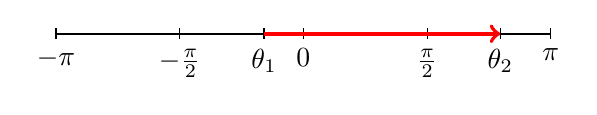
\begin{tikzpicture}
    \draw[thick] (-3.14159, 0) -- (3.14159, 0);
    \draw (-3.14159 cm, 2 pt) -- (-3.14159 cm, -2 pt) node[anchor=north] {$-\pi$};
    \draw (-1.5708 cm, 2 pt) -- (-1.5708 cm, -2 pt) node[anchor=north] {$-\frac{\pi}{2}$};
    \draw (-0.5 cm, 2 pt) -- (-0.5 cm, -2 pt) node[anchor=north] {$\theta_1$};
    \draw (0 cm, 2 pt) -- (0 cm, -2 pt) node[anchor=north] {$0$};
    \draw (1.5708 cm, 2 pt) -- (1.5708 cm, -2 pt) node[anchor=north] {$\frac{\pi}{2}$};
    \draw (2.5 cm, 2 pt) -- (2.5 cm, -2 pt) node[anchor=north] {$\theta_2$};
    \draw (3.14159 cm, 2 pt) -- (3.14159 cm, -2 pt) node[anchor=north] {$\pi$};
    \draw[line width=0.5 mm, red, ->] (-0.5, 0) -- (2.5, 0);
    \end{tikzpicture}
    \caption{Go directly from $\theta_1$ to $\theta_2$}
\end{subfigure}
\hfill
\begin{subfigure}[b]{0.475\textwidth}
    \centering
    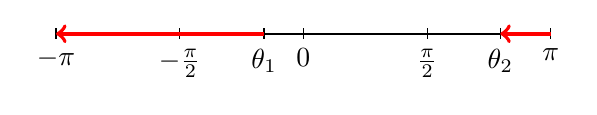
\begin{tikzpicture}
    \draw[thick] (-3.14159, 0) -- (3.14159, 0);
    \draw (-3.14159 cm, 2 pt) -- (-3.14159 cm, -2 pt) node[anchor=north] {$-\pi$};
    \draw (-1.5708 cm, 2 pt) -- (-1.5708 cm, -2 pt) node[anchor=north] {$-\frac{\pi}{2}$};
    \draw (-0.5 cm, 2 pt) -- (-0.5 cm, -2 pt) node[anchor=north] {$\theta_1$};
    \draw (0 cm, 2 pt) -- (0 cm, -2 pt) node[anchor=north] {$0$};
    \draw (1.5708 cm, 2 pt) -- (1.5708 cm, -2 pt) node[anchor=north] {$\frac{\pi}{2}$};
    \draw (2.5 cm, 2 pt) -- (2.5 cm, -2 pt) node[anchor=north] {$\theta_2$};
    \draw (3.14159 cm, 2 pt) -- (3.14159 cm, -2 pt) node[anchor=north] {$\pi$};
    \draw[line width=0.5 mm, red, <-] (-3.14159, 0) -- (-0.5, 0);
    \draw[line width=0.5 mm, red, <-] (2.5, 0) -- (3.14159, 0);
    \end{tikzpicture}
    \caption{Go from $\theta_1$ to $-\pi$, then from $\pi$ to  $\theta_2$}
\end{subfigure}
\caption{Interpolation of angles on a linear axis}
\label{fig:linear_axis}
\end{figure}

Any angle of rotation of $-\pi < \theta \le \pi$ can be represented by a point on the unit circle at $(\cos(\theta),\ \sin(\theta))$, which means that going from one angle to the other during the interpolation is the same as moving from one point to the other along the arc of the unit circle. The two possible ways of interpolating angles are thus represented by the two arcs connecting the points, one being longer than the other.

\begin{figure}[h!]
\centering
\begin{subfigure}[b]{0.475\textwidth}
    \centering
    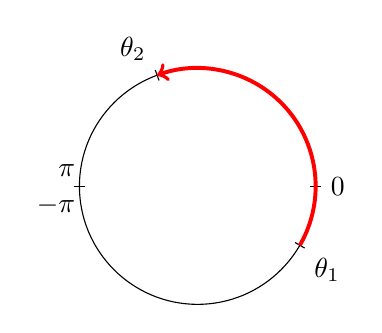
\begin{tikzpicture}
    \draw (0,0) circle (1.5 cm);
    \draw (1.5 cm - 2 pt, 0) -- (1.5 cm + 2 pt, 0) node[anchor=west] {$0$};
    \draw (-1.5 cm - 2 pt, 0) -- (-1.5 cm + 2 pt, 0) node[anchor=south east] {$\pi$};
    \draw (-1.5 cm - 2 pt, 0) -- (-1.5 cm + 2 pt, 0) node[anchor=north east] {$-\pi$};
    \draw (330:1.5 cm - 2 pt) -- (330:1.5 cm + 2 pt) node[anchor=north west] {$\theta_1$};
    \draw (110:1.5 cm - 2 pt) -- (110:1.5 cm + 2 pt) node[anchor=south east] {$\theta_2$};
    \draw[line width=0.5 mm, red, ->] (330:1.5 cm) arc (-30:110:1.5 cm);
    \end{tikzpicture}
    \caption{Shorter arc connecting $\theta_1$ and $\theta_2$}
\end{subfigure}
\hfill
\begin{subfigure}[b]{0.475\textwidth}
    \centering
    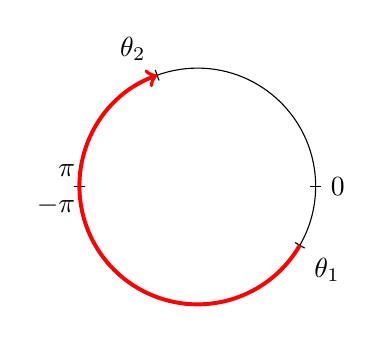
\begin{tikzpicture}
    \draw (0,0) circle (1.5 cm);
    \draw (1.5 cm - 2 pt, 0) -- (1.5 cm + 2 pt, 0) node[anchor=west] {$0$};
    \draw (-1.5 cm - 2 pt, 0) -- (-1.5 cm + 2 pt, 0) node[anchor=south east] {$\pi$};
    \draw (-1.5 cm - 2 pt, 0) -- (-1.5 cm + 2 pt, 0) node[anchor=north east] {$-\pi$};
    \draw (330:1.5 cm - 2 pt) -- (330:1.5 cm + 2 pt) node[anchor=north west] {$\theta_1$};
    \draw (110:1.5 cm - 2 pt) -- (110:1.5 cm + 2 pt) node[anchor=south east] {$\theta_2$};
    \draw[line width=0.5 mm, red, <-] (110:1.5 cm) arc (110:330:1.5 cm);
    \end{tikzpicture}
    \caption{Longer arc connecting $\theta_1$ and $\theta_2$}
\end{subfigure}
\caption{Interpolation of angles on the unit circle}
\label{fig:circular_axis}
\end{figure}

Using this unit circle representation, we can then visualize four different ways of interpolating two angles depending on the values of the two angles. These four cases are shown in Figure \ref{fig:interpolation_situations}.

\begin{figure}[h!]
\centering
\begin{subfigure}[b]{0.475\textwidth}
    \centering
    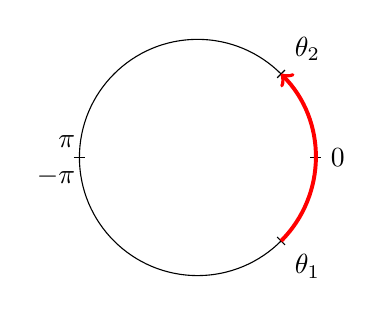
\begin{tikzpicture}
    \draw (0,0) circle (1.5 cm);
    \draw (1.5 cm - 2 pt, 0) -- (1.5 cm + 2 pt, 0) node[anchor=west] {$0$};
    \draw (-1.5 cm - 2 pt, 0) -- (-1.5 cm + 2 pt, 0) node[anchor=south east] {$\pi$};
    \draw (-1.5 cm - 2 pt, 0) -- (-1.5 cm + 2 pt, 0) node[anchor=north east] {$-\pi$};
    \draw (-45:1.5 cm - 2 pt) -- (-45:1.5 cm + 2 pt) node[anchor=north west] {$\theta_1$};
    \draw (45:1.5 cm - 2 pt) -- (45:1.5 cm + 2 pt) node[anchor=south west] {$\theta_2$};
    \draw[line width=0.5 mm, red, ->] (-45:1.5 cm) arc (-45:45:1.5 cm);
    \end{tikzpicture}
    \caption{$\theta_1 < \theta_2$ and $\theta_2 - \theta_1 <= \pi$}
\end{subfigure}
\hfill
\begin{subfigure}[b]{0.475\textwidth}
    \centering
    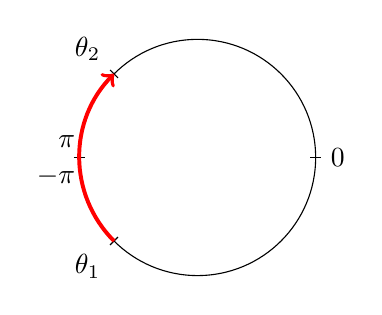
\begin{tikzpicture}
    \draw (0,0) circle (1.5 cm);
    \draw (1.5 cm - 2 pt, 0) -- (1.5 cm + 2 pt, 0) node[anchor=west] {$0$};
    \draw (-1.5 cm - 2 pt, 0) -- (-1.5 cm + 2 pt, 0) node[anchor=south east] {$\pi$};
    \draw (-1.5 cm - 2 pt, 0) -- (-1.5 cm + 2 pt, 0) node[anchor=north east] {$-\pi$};
    \draw (225:1.5 cm - 2 pt) -- (225:1.5 cm + 2 pt) node[anchor=north east] {$\theta_1$};
    \draw (135:1.5 cm - 2 pt) -- (135:1.5 cm + 2 pt) node[anchor=south east] {$\theta_2$};
    \draw[line width=0.5 mm, red, <-] (135:1.5 cm) arc (135:225:1.5 cm);
    \end{tikzpicture}
    \caption{$\theta_1 < \theta_2$ and $\theta_2 - \theta_1 > \pi$}
\end{subfigure}
\vskip\baselineskip
\begin{subfigure}[b]{0.475\textwidth}
    \centering
    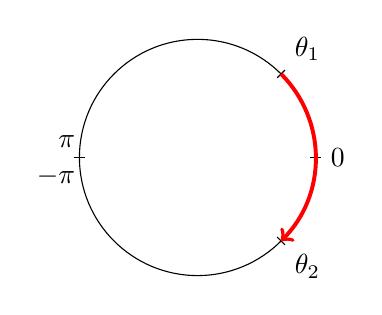
\begin{tikzpicture}
    \draw (0,0) circle (1.5 cm);
    \draw (1.5 cm - 2 pt, 0) -- (1.5 cm + 2 pt, 0) node[anchor=west] {$0$};
    \draw (-1.5 cm - 2 pt, 0) -- (-1.5 cm + 2 pt, 0) node[anchor=south east] {$\pi$};
    \draw (-1.5 cm - 2 pt, 0) -- (-1.5 cm + 2 pt, 0) node[anchor=north east] {$-\pi$};
    \draw (-45:1.5 cm - 2 pt) -- (-45:1.5 cm + 2 pt) node[anchor=north west] {$\theta_2$};
    \draw (45:1.5 cm - 2 pt) -- (45:1.5 cm + 2 pt) node[anchor=south west] {$\theta_1$};
    \draw[line width=0.5 mm, red, <-] (-45:1.5 cm) arc (-45:45:1.5 cm);
    \end{tikzpicture}
    \caption{$\theta_1 > \theta_2$ and $\theta_1 - \theta_2 < \pi$}
\end{subfigure}
\hfill
\begin{subfigure}[b]{0.475\textwidth}
    \centering
    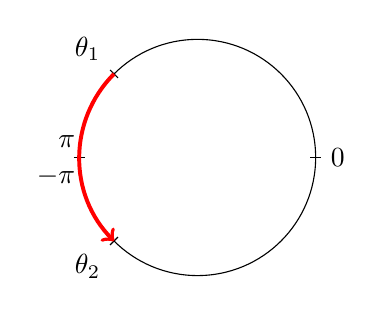
\begin{tikzpicture}
    \draw (0,0) circle (1.5 cm);
    \draw (1.5 cm - 2 pt, 0) -- (1.5 cm + 2 pt, 0) node[anchor=west] {$0$};
    \draw (-1.5 cm - 2 pt, 0) -- (-1.5 cm + 2 pt, 0) node[anchor=south east] {$\pi$};
    \draw (-1.5 cm - 2 pt, 0) -- (-1.5 cm + 2 pt, 0) node[anchor=north east] {$-\pi$};
    \draw (225:1.5 cm - 2 pt) -- (225:1.5 cm + 2 pt) node[anchor=north east] {$\theta_2$};
    \draw (135:1.5 cm - 2 pt) -- (135:1.5 cm + 2 pt) node[anchor=south east] {$\theta_1$};
    \draw[line width=0.5 mm, red, ->] (135:1.5 cm) arc (135:225:1.5 cm);
    \end{tikzpicture}
    \caption{$\theta_1 > \theta_2$ and $\theta_1 - \theta_2 >= \pi$}
\end{subfigure}
\caption{Four different situations when interpolating angles of rotation}
\label{fig:interpolation_situations}
\end{figure}

Computing the interpolated angle is then done using one of the four equations below, depending on in which of the cases shown in Figure \ref{fig:interpolation_situations} we currently are.

\[
    \theta = 
    \begin{cases}
        \text{case a: } \theta_1 + (\theta_2 - \theta_1)*ratio \\
        \text{case b: } \theta_2 + (2\pi + \theta_1 - \theta_2)*(1 - ratio) \\
        \text{case c: } \theta_2 + (\theta_1 - \theta_2)*(1 - ratio) \\
        \text{case d: } \theta_1 + (2\pi + \theta_2 - \theta_1)*ratio \\
    \end{cases}
\]

Finally, if the resulting angle is larger than $\pi$, we subtract $2\pi$ from it to keep the angle between $-\pi$ and $\pi$.

As a last remark, if the difference between the start and end angle is exactly $\pi$, we always interpolate in a counter-clockwise manner. This means that when $\theta_1 < \theta_2$, the interpolation goes through $0$, and otherwise the interpolation goes through $\pi$.

\begin{figure}[h!]
\centering
\begin{subfigure}[b]{0.475\textwidth}
    \centering
    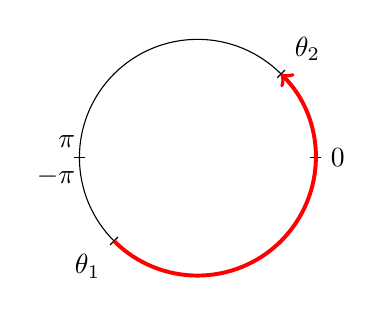
\begin{tikzpicture}
    \draw (0,0) circle (1.5 cm);
    \draw (1.5 cm - 2 pt, 0) -- (1.5 cm + 2 pt, 0) node[anchor=west] {$0$};
    \draw (-1.5 cm - 2 pt, 0) -- (-1.5 cm + 2 pt, 0) node[anchor=south east] {$\pi$};
    \draw (-1.5 cm - 2 pt, 0) -- (-1.5 cm + 2 pt, 0) node[anchor=north east] {$-\pi$};
    \draw (-135:1.5 cm - 2 pt) -- (-135:1.5 cm + 2 pt) node[anchor=north east] {$\theta_1$};
    \draw (45:1.5 cm - 2 pt) -- (45:1.5 cm + 2 pt) node[anchor=south west] {$\theta_2$};
    \draw[line width=0.5 mm, red, ->] (-135:1.5 cm) arc (-135:45:1.5 cm);
    \end{tikzpicture}
    \caption{$\theta_1 < \theta_2$ and $\theta_2 - \theta_1 = \pi$}
\end{subfigure}
\hfill
\begin{subfigure}[b]{0.475\textwidth}
    \centering
    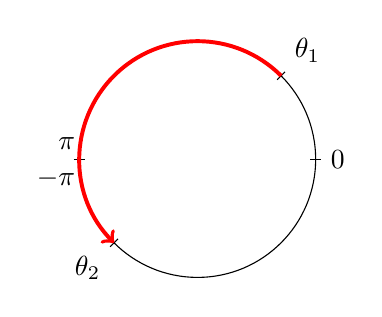
\begin{tikzpicture}
    \draw (0,0) circle (1.5 cm);
    \draw (1.5 cm - 2 pt, 0) -- (1.5 cm + 2 pt, 0) node[anchor=west] {$0$};
    \draw (-1.5 cm - 2 pt, 0) -- (-1.5 cm + 2 pt, 0) node[anchor=south east] {$\pi$};
    \draw (-1.5 cm - 2 pt, 0) -- (-1.5 cm + 2 pt, 0) node[anchor=north east] {$-\pi$};
    \draw (225:1.5 cm - 2 pt) -- (225:1.5 cm + 2 pt) node[anchor=north east] {$\theta_2$};
    \draw (45:1.5 cm - 2 pt) -- (45:1.5 cm + 2 pt) node[anchor=south west] {$\theta_1$};
    \draw[line width=0.5 mm, red, ->] (45:1.5 cm) arc (45:225:1.5 cm);
    \end{tikzpicture}
    \caption{$\theta_1 > \theta_2$ and $\theta_1 - \theta_2 = \pi$}
\end{subfigure}
\caption{Interpolation of a 180 degree rotation}
\label{fig:180_rotation}
\end{figure}

\subsection{Interpolate Long}
\label{section:interpolate_long}

The \textit{interpolate long} function does the same as the \textit{interpolate} function, except that during the interpolation of the angles, it always takes the longest arc instead of the smallest. This function will be useful in Section \ref{section:normalization}, when normalizing a tgeometryseq.

\subsection{Combine}
\label{section:combine}

The \textit{combine} function essentially does an addition of two rtransform value. With the input rtransform objects being written as $(v_1^x,\ v_1^y,\ \theta_1)$ and $(v_2^x,\ v_2^y,\ \theta_2)$, the resulting rtransform is computed as:

\begin{align*}
        & v^x = v_1^x + v_2^x \\
        & v^y = v_1^y + v_2^y \\
        & \theta = 
        \begin{cases}
            \theta_1 + \theta_2 - 2\pi,\ \text{if } \pi < \theta_1 + \theta_2 \\
            \theta_1 + \theta_2 + 2\pi,\ \text{if } \theta_1 + \theta_2 \le -\pi \\
            \theta_1 + \theta_2,\ \text{otherwise}
        \end{cases}
\end{align*}

This function is used when we need to change the start/reference region of the rtransform, for example when we need to merge two tgeometryi. 

\begin{flalign*}
    & \text{merge(}\{\mathcal{R}_0@t_0,\ \mathcal{T}_1@t_1\},\ \{\mathcal{R}_0'@t_2,\ \mathcal{T}_1'@t_3\}) &&\\
    & \text{-- -- }\ '\{\mathcal{R}_0@t_0,\ \mathcal{T}_1@t_1,\ \mathcal{T}_2@t_2,\ \mathcal{T}_3@t_3\}'\ \text{-- --} &&\\
\end{flalign*}

In this case, computing $\mathcal{T}_3$ requires us to \textit{combine} $\mathcal{T}_1'$ and the newly computed $\mathcal{T}_2$.

\subsection{Difference}
\label{section:diff}

The \textit{diff} function is similar to the compute function, except that it does the difference between the first and the second input argument, instead of doing an addition.

\begin{align*}
        & v^x = v_2^x - v_1^x \\
        & v^y = v_2^y - v_1^y \\
        & \theta = 
        \begin{cases}
            \theta_2 - \theta_1 - 2\pi,\ \text{if } \pi < \theta_2 - \theta_1 \\
            \theta_2 - \theta_1 + 2\pi,\ \text{if } \theta_2 - \theta_1 \le -\pi \\
            \theta_2 - \theta_1,\ \text{otherwise}
        \end{cases}
\end{align*}

When we want to know what the transformation is between two instants, when both instants are saved as rtransforms relative to a third instant, we can use simply do the difference between the rtransform of the final instant and the rtransform of the initial instant to get the result.

For example, if we have a tgeometryi with 3 instants $'\{\mathcal{R}_0@t_0,\ \mathcal{T}_1@t_1,\ \mathcal{T}_2@t_2\}'$, and we want to get the transformation to go from the second instant to the third, we can apply $\textit{diff}(\mathcal{T}_2,\ \mathcal{T}_1)$.